\documentclass[conference]{IEEEtran}
\usepackage{cite}
\usepackage{amsmath,amssymb}
\usepackage{graphicx}
\usepackage{booktabs}
\usepackage{array}
\usepackage[table]{xcolor}
\usepackage{url}
\graphicspath{{../outputs/figures/}}
\definecolor{answer}{RGB}{255,246,214}

\begin{document}

\title{Unsupervised Detection of Genesis Outliers in Mars HiRISE Orbital Imagery with a Two-Stage
Residual Autoencoder and Latent-Space Isolation Forest}

\author{\IEEEauthorblockN{Team OrbitIQ}
\IEEEauthorblockA{National Students' Space Challenge (NSSC) 2026 --- Data Analytics\\
Indian Institute of Technology Kharagpur, India}}

\maketitle

\begin{abstract}
We present an end-to-end, fully unsupervised pipeline that finds tampered or foreign crops (``Genesis
Outliers'': spliced terrain, terrestrial content and synthetic sensor artefacts) among 10{,}422
HiRISE crops of $227\times227$ pixels, without labels and without pretrained networks. A convolutional
autoencoder trained from scratch compresses every crop into a 256-d scene code; a second autoencoder
compresses the first one's reconstruction residual into a 64-d code, and the concatenated 320-d latent
is scored by an Isolation Forest. A robust modified $z$-score rule on the observed score distribution
flags \textbf{48 crops (0.46\,\%)}. Two engineering steps were decisive:
masking map-projection no-data wedges, which in the first two model versions had made about 96\,\% of
all flags border crops, and the residual code, which raised the mean AUROC on a benchmark of 2{,}400
planted splices, glitches and man-made textures from 0.735 to 0.775 (raw-pixel Isolation Forest:
0.45). Four of the six highest-scoring crops are Earth-like aerial images; reconstruction-error
heatmaps separate their diffuse, whole-frame failure from the concentrated, relief-following error of
rare genuine terrain, and a metadata join attributes much of the remaining tail to two north-polar
observations.
\end{abstract}

\begin{IEEEkeywords}
anomaly detection, convolutional autoencoder, isolation forest, HiRISE, Mars, unsupervised learning,
novelty detection, interpretability
\end{IEEEkeywords}

\section{Introduction}
The HiRISE camera on the Mars Reconnaissance Orbiter has produced one of the richest image archives of
another planet \cite{mcewen2007}. Rare frames that do not belong must be found without anyone labelling
them, which mirrors the workflow of a planetary-imaging pipeline. The competition dataset \cite{doran2020}
contains an undisclosed number of injected outliers of three classes (\emph{semantic splicing},
\emph{domain-shifted terrestrial content} and \emph{synthetic sensor artefacts}) at unknown positions.

Our contributions are: (i) a from-scratch convolutional autoencoder (CAE) with a masked structural loss
and a second-stage residual code; (ii) an Isolation Forest (IF) novelty engine on the 1-D latent
vectors with a statistically justified, count-free threshold; (iii) a metadata-grounded location
analysis; (iv) reconstruction-error heatmaps with quantitative descriptors; (v) a documented iteration
journal of six versions; and (vi) a planted-fakes benchmark that compares models without touching the
hidden labels or tuning the threshold. Table~\ref{tab:final} summarises the final answers.

\begin{table}[!t]
\centering
\caption{Final Answers}
\label{tab:final}
\renewcommand{\arraystretch}{1.15}
\colorbox{answer}{\begin{tabular}{@{}>{\raggedright\arraybackslash}p{0.25\columnwidth}>{\raggedright\arraybackslash}p{0.65\columnwidth}@{}}
\textbf{Final model} & v6: two-stage CAE trained from scratch; a fixed-length 320-dimensional latent vector (a 256-d scene code from stage~1 concatenated with a 64-d code of its reconstruction residual) \\
\textbf{Loss} & stage 1: $0.84(1-\mathrm{SSIM}) + 0.16L_1 + 0.1L_{\nabla}$; stage 2: MSE $+\,0.5\,L_1$; no-data masked \\
\textbf{Novelty Score} & IF $s(x,n)$ on the latent, 500 trees $\times$ 5 seeds; higher = more anomalous \\
\textbf{Threshold} & modified $z > 3.5$ $\Rightarrow$ $\tau = \mathbf{0.5251}$ \\
\textbf{Flagged} & \textbf{48} of 10{,}422 crops (0.46\,\%) \\
\textbf{Top-5 (Phase 3)} & 06476, 06963, 07971, 03383, 07701 \\
\textbf{Location} & 2 enriched observations, both polar \\
\textbf{Fusion} & 54 vs 48 flagged (Jaccard 0.82) \\
\end{tabular}}
\end{table}

\section{Data and Pre-processing}
The dataset holds 10{,}422 single-channel $227\times227$ JPEG crops from 172 source observations;
every crop maps to exactly one \texttt{source\_image\_id} with metadata (latitude, longitude, sun angle,
season, resolution). Pixel values span 0--255 and are rescaled to $[0,1]$. A sanity pass revealed that
\textbf{19.7\,\% of crops contain a solid-black no-data wedge}, the map-projected edge of the HiRISE strip
(Fig.~\ref{fig:nodata}): normal data, but the highest-contrast edges in the dataset.

From v3 onwards each crop receives a no-data mask: near-black ($\le 5$) regions that survive a
$5\times5$ morphological opening, touch the crop border and cover at least 0.5\,\% of the crop, dilated by
2\,px for JPEG ringing. The opening deliberately keeps thin interior dark lines, which may themselves be
injected artefacts. Masked pixels are filled with the crop's valid-pixel median and excluded from every
loss term, metric and heatmap.
\begin{figure*}[!t]
\centering
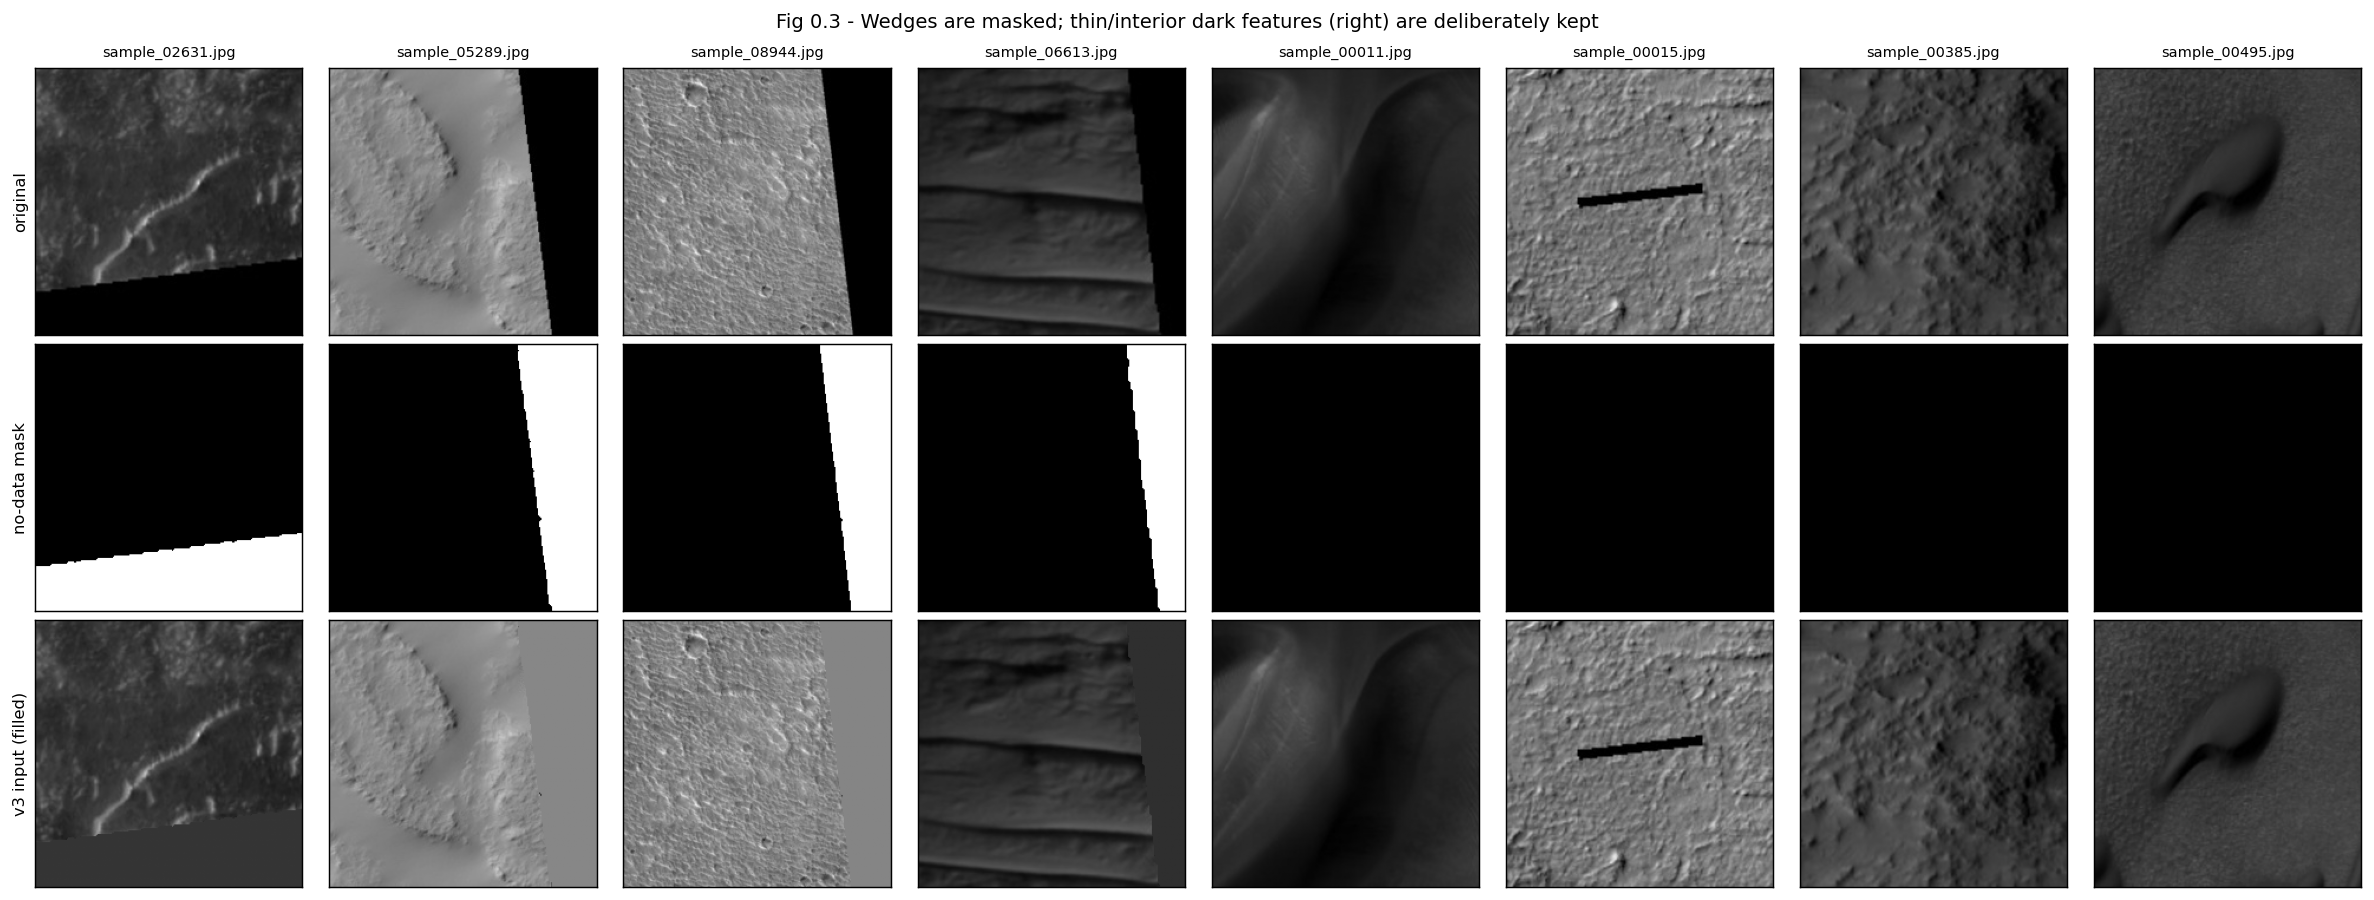
\includegraphics[width=0.8\textwidth]{fig02b_nodata_masks.png}
\caption{No-data masking. Top: originals; middle: mask; bottom: model input. Projection wedges (left) are masked; thin interior dark features (right) are deliberately kept.}
\label{fig:nodata}
\end{figure*}


\section{Method}
\subsection{Stage 1: Convolutional Autoencoder}
The encoder applies five stride-2 $3\times3$ convolutions (32, 64, 128, 256, 256 channels, BatchNorm,
LeakyReLU), mapping $227\to114\to57\to29\to15\to8$; a linear layer maps the flattened $8\times8\times256$
map to the scene code $\mathbf{z}_1\in\mathbb{R}^{256}$. The decoder mirrors it with transposed
convolutions to $256\times256$, centre-cropped to $227\times227$ with a sigmoid output (11.1\,M parameters).
All networks are randomly initialised and trained only on the competition crops (AdamW, one-cycle
learning rate $10^{-3}$, batch 64, 30 epochs, flip augmentation, bf16 autocast, seed 42) \cite{hinton2006,loshchilov2019}.

\subsection{Reconstruction Loss}
With a validity map $w$ (0 on no-data pixels) and $\langle\cdot\rangle_w$ the $w$-weighted mean,
\begin{equation}
\mathcal{L}_1 = 0.84\big(1-\langle \mathrm{SSIM}(x,\hat{x})\rangle_w\big) + 0.16\,\langle |x-\hat{x}|\rangle_w + 0.1\,\mathcal{L}_{\nabla},
\end{equation}
where SSIM \cite{wang2004} uses an $11\times11$ Gaussian window ($\sigma=1.5$), the 0.84/0.16 split follows
\cite{zhao2017}, and $\mathcal{L}_{\nabla}$ is the $L_1$ distance between finite differences. SSIM
penalises lost local structure that MSE averages away, $L_1$ anchors absolute albedo and the gradient
term protects ridgelines and crater rims. No perceptual loss is used: any perceptual network would be
pretrained.

\subsection{Stage 2: Residual Code}
A second autoencoder of the same design with a 64-d bottleneck is trained (MSE $+\,0.5\,L_1$ on valid
pixels) on stage~1's amplified signed residual $r = 128 + 127\,\mathrm{clip}(4(x-\hat{x}),-1,1)$. The
final latent is $\mathbf{z} = [\mathbf{z}_1;\mathbf{z}_2]\in\mathbb{R}^{320}$: $\mathbf{z}_1$ describes
\emph{what kind of terrain} a crop shows, $\mathbf{z}_2$ \emph{what stage~1 could not explain}.

\subsection{Latent Dimensionality}
We trained stage~1 with $d\in\{64,128,256,512\}$ for 12 epochs (Table~\ref{tab:sweep}). Fidelity saturates
(SSIM $+0.004$ from 256 to 512) and the number of principal components holding 90\,\% of latent variance
grows sub-linearly: the extra coordinates of $d=512$ are largely redundant and dilute the IF's uniformly
random feature choice. The tail ratio $(q_{99.9}-\mathrm{median})/\mathrm{MAD}$ of the Novelty Scores is
nearly flat across $d$, so it serves only as a sanity check; we choose $d=256$ on fidelity and effective
dimensionality.

\begin{table}[!t]
\centering
\caption{Stage-1 latent-size sweep (12-epoch schedule, single seed)}
\label{tab:sweep}
\footnotesize
\begin{tabular}{@{}cccc@{}}
\toprule
$d$ & SSIM & PCs (90\,\%) & tail ratio \\
\midrule
64 & 0.682 & 30 & 10.89 \\
128 & 0.678 & 8 & 9.51 \\
\rowcolor{yellow!20}256 & 0.692 & 85 & 11.05 \\
512 & 0.696 & 109 & 10.49 \\
\bottomrule
\end{tabular}
\end{table}

\subsection{Isolation Forest Novelty Score}
An IF \cite{liu2008} with 500 trees and sub-sample size $\psi=256$ is fitted on the latents of all crops;
five forests with different seeds are averaged (rank correlation between independent forests 0.98). With
$h(x)$ the path length and $c(\psi)$ its expected value,
\begin{equation}
s(x,\psi) = 2^{-\mathbb{E}[h(x)]/c(\psi)} \in (0,1].
\end{equation}
scikit-learn's \texttt{score\_samples} returns $-s$; we negate it, so the \textbf{Novelty Score is $s$ and
higher means more anomalous} (correlation $-0.98$ with \texttt{decision\_function}). \texttt{contamination}
stays at \texttt{"auto"}; it only affects \texttt{predict()}, which is never called, so the anomaly count
is independent of any assumed contamination fraction.

\subsection{Statistical Threshold}
The final scores are not Gaussian (skewness 0.75, excess kurtosis 0.65,
D'Agostino $K^2=885$, $p\approx0$ \cite{dagostino1971}), and $\mu,\sigma$ are inflated by the very tail being
sought. We use the modified $z$-score of Iglewicz and Hoaglin \cite{iglewicz1993},
\begin{equation}
M_i = 0.6745\,\frac{s_i-\tilde{s}}{\mathrm{MAD}}, \qquad \text{flag } M_i > 3.5,
\end{equation}
whose median $\tilde{s}$ and MAD have a 50\,\% breakdown point, so the outliers cannot move the boundary.
Under a Gaussian bulk with this scale about 2.4 of 10{,}422 normal crops would exceed it by chance;
the real bulk is right-skewed, so this is a lower bound. Table~\ref{tab:thr} compares the alternatives.
Because the distribution is unimodal, the two-component GMM splits the skewed bulk itself and the Kneedle
elbow \cite{satopaa2011} of the whole sorted curve marks the onset of the ordinary right skew; both fall
inside the body of the distribution. The robust rule (48) lies between the classical $\mu+3\sigma$
cross-check (82) and the same rule applied to log-scores (22, skew 0.54); all three sit in the final
steep rise of the sorted scores (Fig.~\ref{fig:thr}). For $k=3, 3.5, 4, 5$ the count is 97, 48, 24, 1;
$k$ is reported, not tuned.

\begin{table}[!t]
\centering
\caption{Candidate thresholds on the final Novelty Scores}
\label{tab:thr}
\footnotesize
\begin{tabular}{@{}lcc@{}}
\toprule
Method & Threshold & Flagged \\
\midrule
\rowcolor{yellow!20}Modified z-score & 0.5251 & 48 \\
Kneedle elbow of sorted scores & 0.4633 & 987 \\
2-component GMM posterior = 0.5 & 0.4291 & 3740 \\
mu + 3 sigma & 0.5145 & 82 \\
\bottomrule
\end{tabular}
\end{table}
\begin{figure*}[!t]
\centering
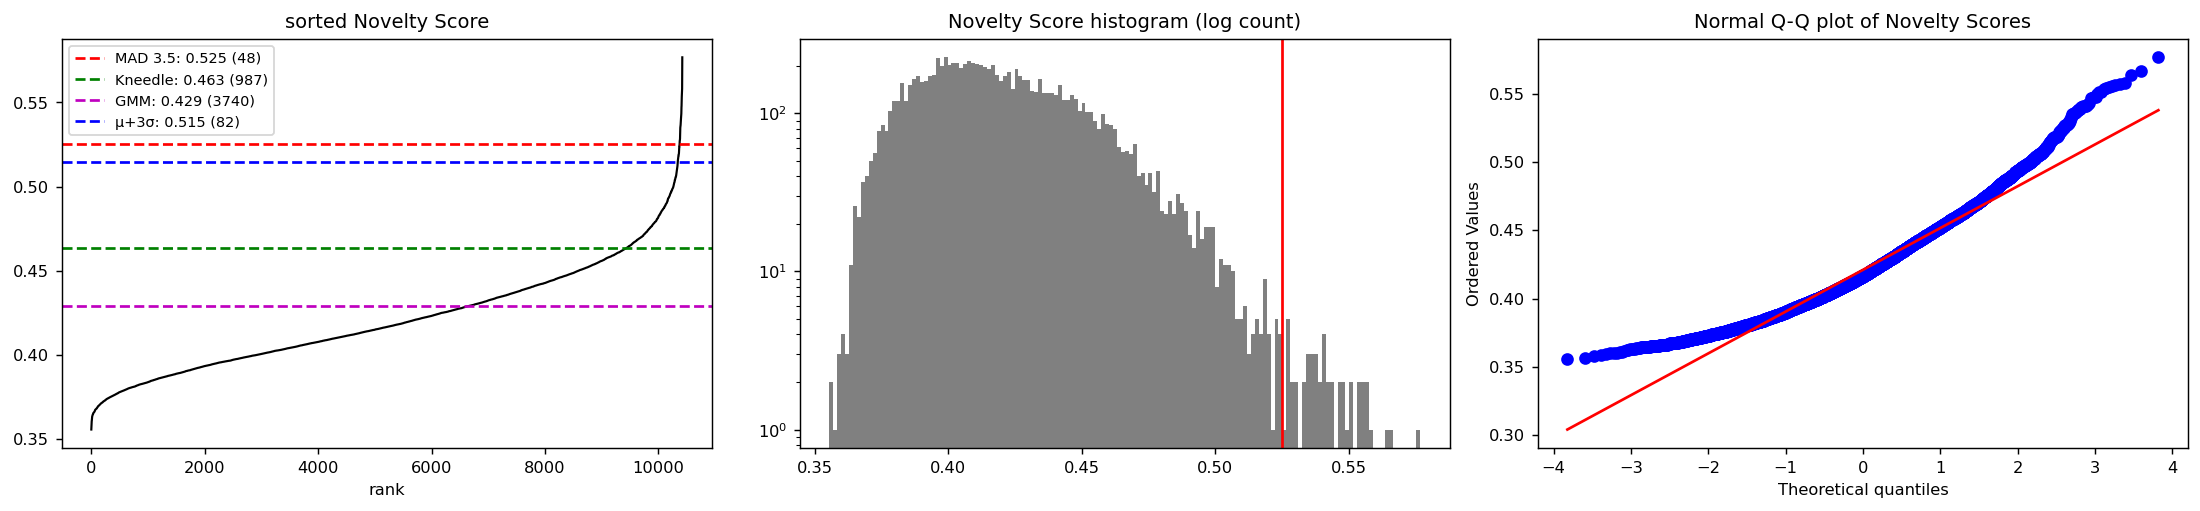
\includegraphics[width=0.92\textwidth]{fig08_threshold_candidates.png}
\caption{Sorted Novelty Scores with candidate thresholds (left), histogram with the final threshold (centre) and normal Q--Q plot (right).}
\label{fig:thr}
\end{figure*}


\section{Engineering Iterations}\label{sec:iter}
Every version uses identical data, schedule, seed and IF (Table~\ref{tab:iter}; full symptom
$\rightarrow$ diagnosis $\rightarrow$ fix journal in \texttt{CHANGELOG.md}).
\textbf{v1 (baseline, MSE).} Reconstructions were blurry and 96\,\% of flags were crops with a no-data wedge
($\rho$(novelty, no-data fraction) $=0.63$, 1{,}596 flags). \textbf{v2 (structural loss)} barely changed
held-out SSIM (0.7053$\rightarrow$0.7065): a 256-float code cannot store the phase of a ripple field, so the
loss was not the binding constraint, and its edge-sensitive terms made the border problem worse.
\textbf{v3 (no-data masking)} removed the nuisance mode ($\rho=0.11$), gave a unimodal score distribution and
brought Earth imagery into the flagged set. \textbf{v4 (spatial $8\times8\times4$ bottleneck)} was rejected: its
coordinates encoded local brightness and it flagged 510 dark or bright scenes. \textbf{v5 (per-crop photometric
normalisation)} was rejected: dividing each crop by its own contrast made planted fakes look \emph{more} typical
(benchmark AUROC 0.40). \textbf{v6 (two-stage residual code)} followed from the benchmark finding that
reconstruction error alone separates fakes better than v3's latent (0.835 vs 0.735) while IF tuning did
not help; it raised the benchmark AUROC to 0.775, $\rho$(novelty, reconstruction error) from 0.44 to 0.57,
reduced the share of flags in the brightness extremes from 58\,\% to 44\,\%, and moved the Earth-like images
found by eye to ranks 1, 3 and 6.

\begin{table}[!t]
\centering
\caption{Model versions: principal components for 90\,\% of latent variance, Spearman $\rho$ of novelty with
no-data fraction, crops flagged, and mean planted-fakes AUROC}
\label{tab:iter}
\setlength{\tabcolsep}{3pt}
\footnotesize
\begin{tabular}{@{}llcccc@{}}
\toprule
Ver. & Change & PCs & $\rho_{\text{nd}}$ & Flags & AUROC \\
\midrule
v1 & Baseline CAE, MSE & 44 & 0.63 & 1596 & 0.497 \\
v2 & SSIM + L1 + gradient loss & 36 & 0.66 & 1985 & 0.504 \\
v3 & No-data masking + fill & 190 & 0.11 & 86 & 0.735 \\
v4 & Spatial $8{\times}8{\times}4$ bottleneck & 139 & 0.07 & 510 & 0.638 \\
v5 & Photometric normalisation & 187 & -0.37 & 0 & 0.395 \\
\rowcolor{yellow!20}v6 & Two-stage residual AE & 238 & 0.10 & 48 & 0.775 \\
\bottomrule
\end{tabular}
\end{table}
\begin{figure*}[!t]
\centering
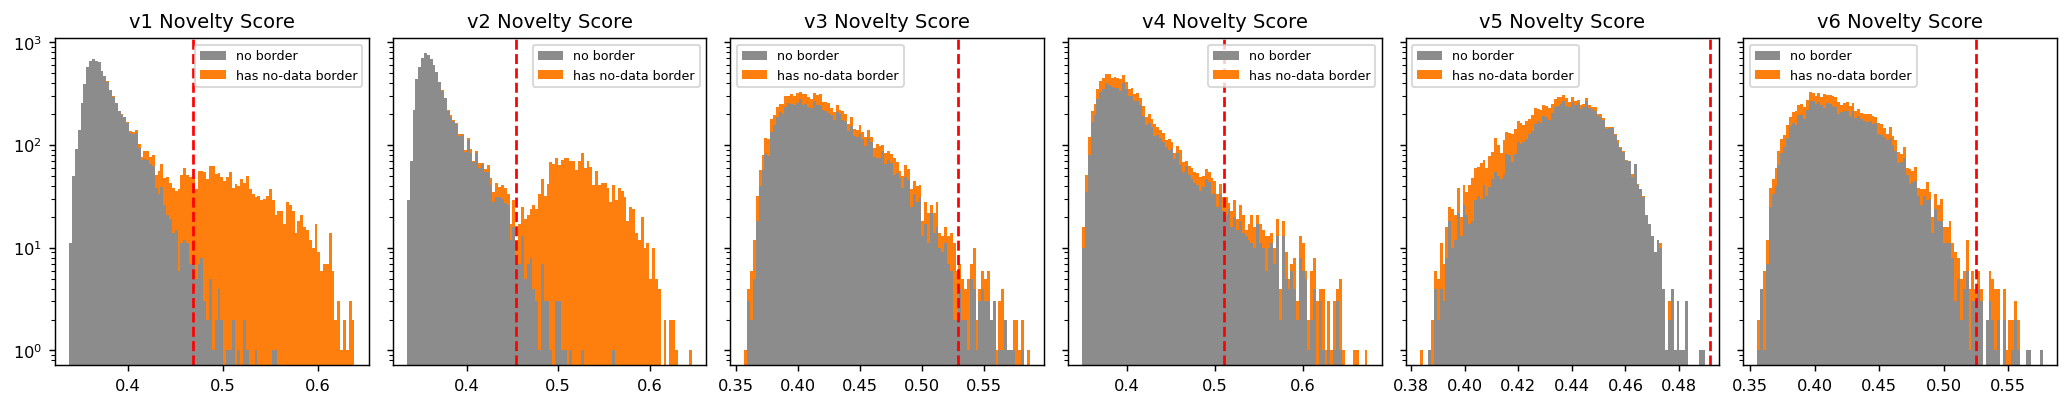
\includegraphics[width=0.92\textwidth]{fig12_versions_hist.png}
\caption{Novelty Score distributions per version; orange marks crops with a no-data wedge. Dashed: modified-$z$ threshold.}
\label{fig:hist}
\end{figure*}


\section{Planted-Fakes Benchmark}\label{sec:bench}
Without ground truth a model cannot be scored directly. We generate 300 instances of each of eight
anomaly types from clean crops (Fig.~\ref{fig:probes}: straight-seam and patch splices; bars, blocks, gain
stripes and line dropouts; periodic and rectilinear man-made textures), pass them through exactly the
same pre-processing as real crops, and score them with each model's IF fitted on the real data only
(Table~\ref{tab:bench}). The threshold rule is never tuned on this benchmark; it only compares models, and
its generators may differ from the organisers' injections.
\begin{figure*}[!t]
\centering
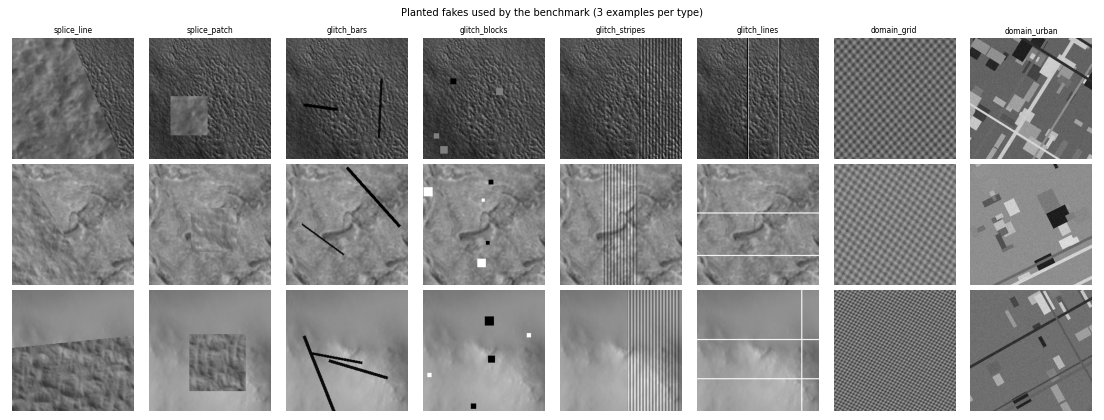
\includegraphics[width=0.92\textwidth]{fig15_probe_examples.png}
\caption{Planted fakes used by the benchmark (three examples per generator).}
\label{fig:probes}
\end{figure*}

\begin{table}[!t]
\centering
\caption{Planted-fakes benchmark: AUROC of fakes against the whole real set (latent + IF), recall at each
model's own threshold, real crops flagged, and reconstruction-error AUROC as a reference}
\label{tab:bench}
\setlength{\tabcolsep}{2.5pt}
\footnotesize
\begin{tabular}{@{}lccccccc@{}}
\toprule
 & \multicolumn{3}{c}{AUROC by class} & AUROC & Rec. & Real & Recon \\
Model & splice & glitch & domain & mean & (\%) & flags & AUROC \\
\midrule
v1 & 0.58 & 0.51 & 0.39 & \textbf{0.497} & 4.6 & 1596 & 0.84 \\
v2 & 0.51 & 0.56 & 0.39 & \textbf{0.504} & 3.2 & 1985 & 0.84 \\
v3 & 0.61 & 0.72 & 0.88 & \textbf{0.735} & 9.5 & 86 & 0.84 \\
v4 & 0.56 & 0.66 & 0.67 & \textbf{0.638} & 6.3 & 510 & 0.83 \\
v5 & 0.45 & 0.33 & 0.47 & \textbf{0.395} & 0.0 & 0 & 0.61 \\
\rowcolor{yellow!20}v6 & 0.65 & 0.77 & 0.91 & \textbf{0.775} & 12.1 & 48 & 0.84 \\
raw pixels & 0.52 & 0.46 & 0.38 & \textbf{0.453} & 1.0 & 485 & -- \\
\bottomrule
\end{tabular}
\end{table}

\section{Results}
\subsection{Latent Space}
PCA (50 components) followed by t-SNE \cite{vandermaaten2008} shows no collapse: a dense core, extended arms
and small islands. Brightness is the dominant organising axis, pixel scale is partly encoded and the no-data
fraction is spread uniformly, confirming the effect of masking. Flagged crops lie mainly on the periphery of
the map (Fig.~\ref{fig:tsne}); these are visual interpretations, not labels.
\begin{figure}[!t]
\centering
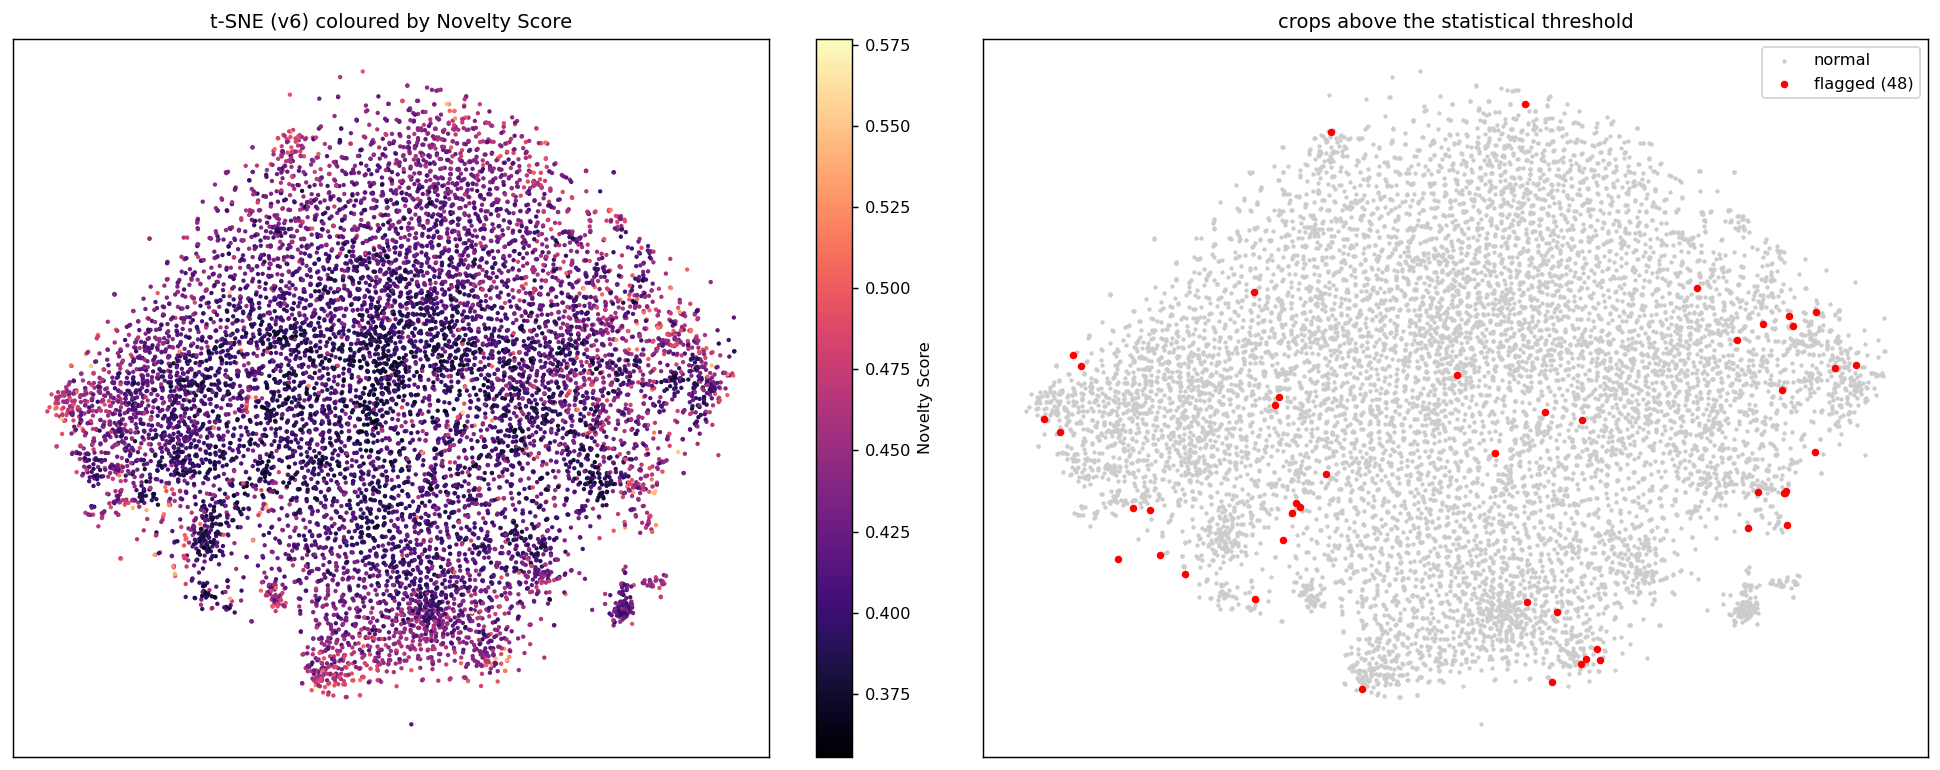
\includegraphics[width=\columnwidth]{fig09_tsne_flagged.png}
\caption{t-SNE of the final latents coloured by Novelty Score (left) and crops above the statistical threshold (right).}
\label{fig:tsne}
\end{figure}

\subsection{Location Analysis}
The metadata is quantised (latitude on a $5^\circ$ grid plus a $90^\circ$ bin; longitude only $0^\circ$ or
$180^\circ$E), so we analyse latitude bands (Fig.~\ref{fig:loc}). Flags span 30 of 172
observations; 2 are significantly enriched (one-sided binomial test, Bonferroni $p<0.05$): SRC\_039 (9 of 16 crops, latitude bin 90$^\circ$) and SRC\_166 (3 of 16 crops, latitude bin 90$^\circ$).
Their bright, finely layered, ice-rich terrain is rare in the training distribution, so the metadata
identifies these flags as a terrain class rather than tampering. The Earth-like crops, by contrast, come from
four different observations at low latitudes, as expected for randomly inserted foreign content. Sun angle
($\rho=-0.03$) and $|$latitude$|$ ($\rho=0.06$) have negligible effect sizes, and flagging is
independent of season ($\chi^2$ $p=0.53$).
\begin{figure*}[!t]
\centering
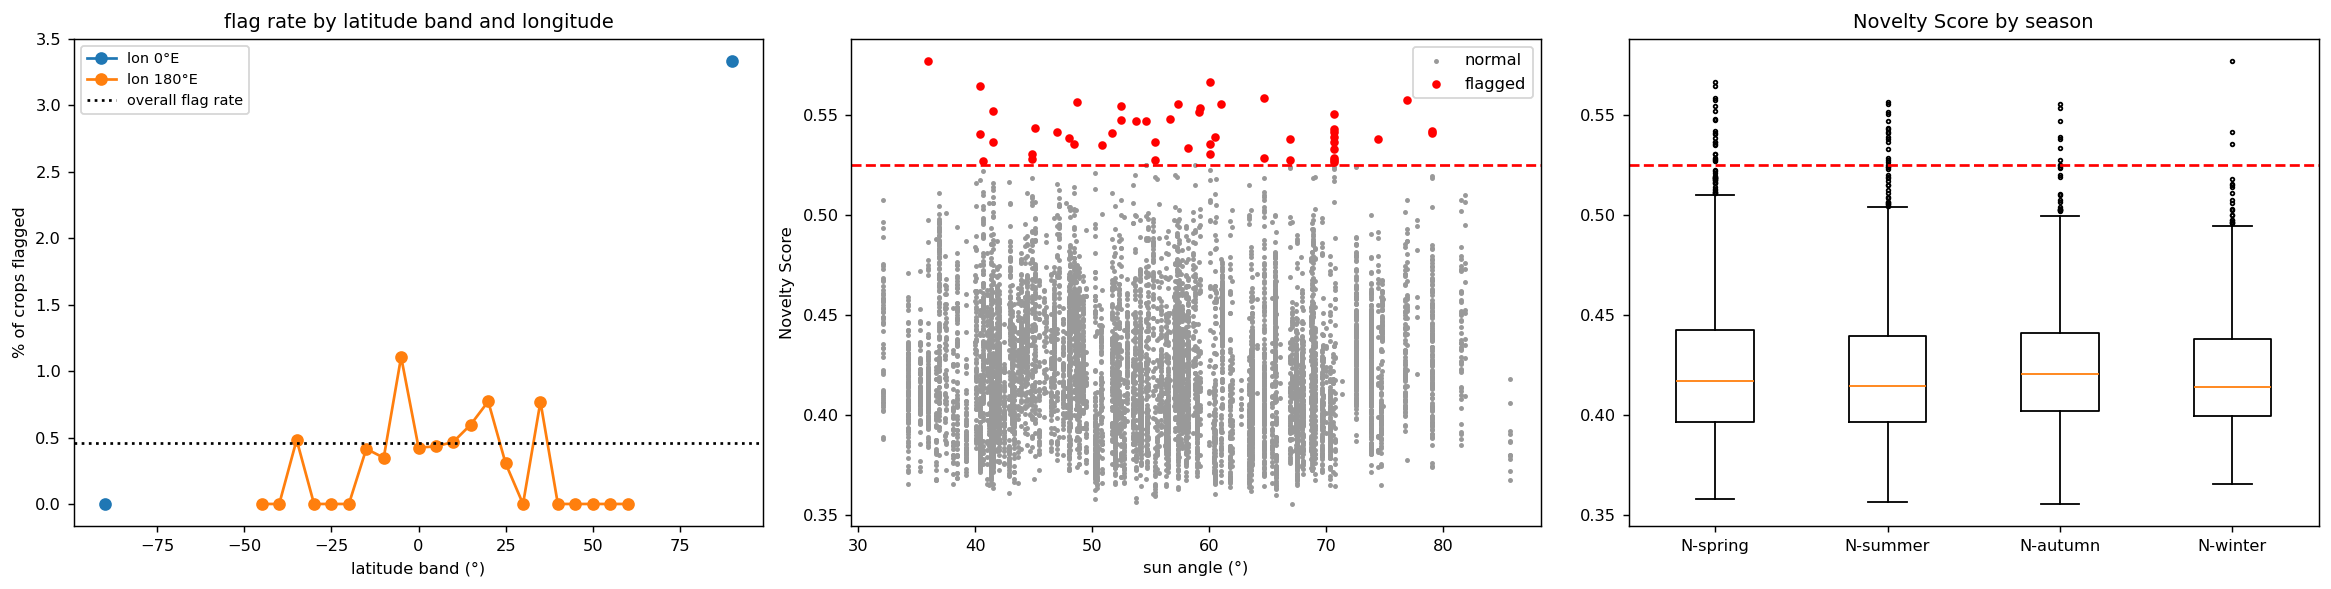
\includegraphics[width=0.92\textwidth]{fig10_location.png}
\caption{Flag rate by latitude band and longitude (left), Novelty Score versus sun angle (centre) and by season (right).}
\label{fig:loc}
\end{figure*}

\subsection{Metadata Fusion}
Concatenating the standardised latent with an encoded metadata vector (z-scored sun angle, sin/cos of
latitude and longitude, log$_2$ resolution, one-hot season) flags 54 crops against 48
(Jaccard 0.82, rank correlation 0.993). Only 10 of 330 fused dimensions are metadata, and all crops of
one observation share identical metadata, so metadata can isolate an unusual observation but never a
single crop: it is most useful for explaining flags after the fact.

\subsection{Reconstruction Heatmaps and Geological Hypotheses}
The five highest-scoring crops \emph{within the thresholded set} are passed back through the stage-1
decoder (Fig.~\ref{fig:hm}); error-map descriptors are reported as percentiles against 500 normal crops
(Table~\ref{tab:top5}). All interpretations are hypotheses. The three crops with \emph{diffuse} error
(concentration at the 2nd--5th percentile) are exactly the three with very high reconstruction error
(0.016--0.030 vs.\ 0.003--0.005), and all three look man-made.
\begin{figure*}[!t]
\centering
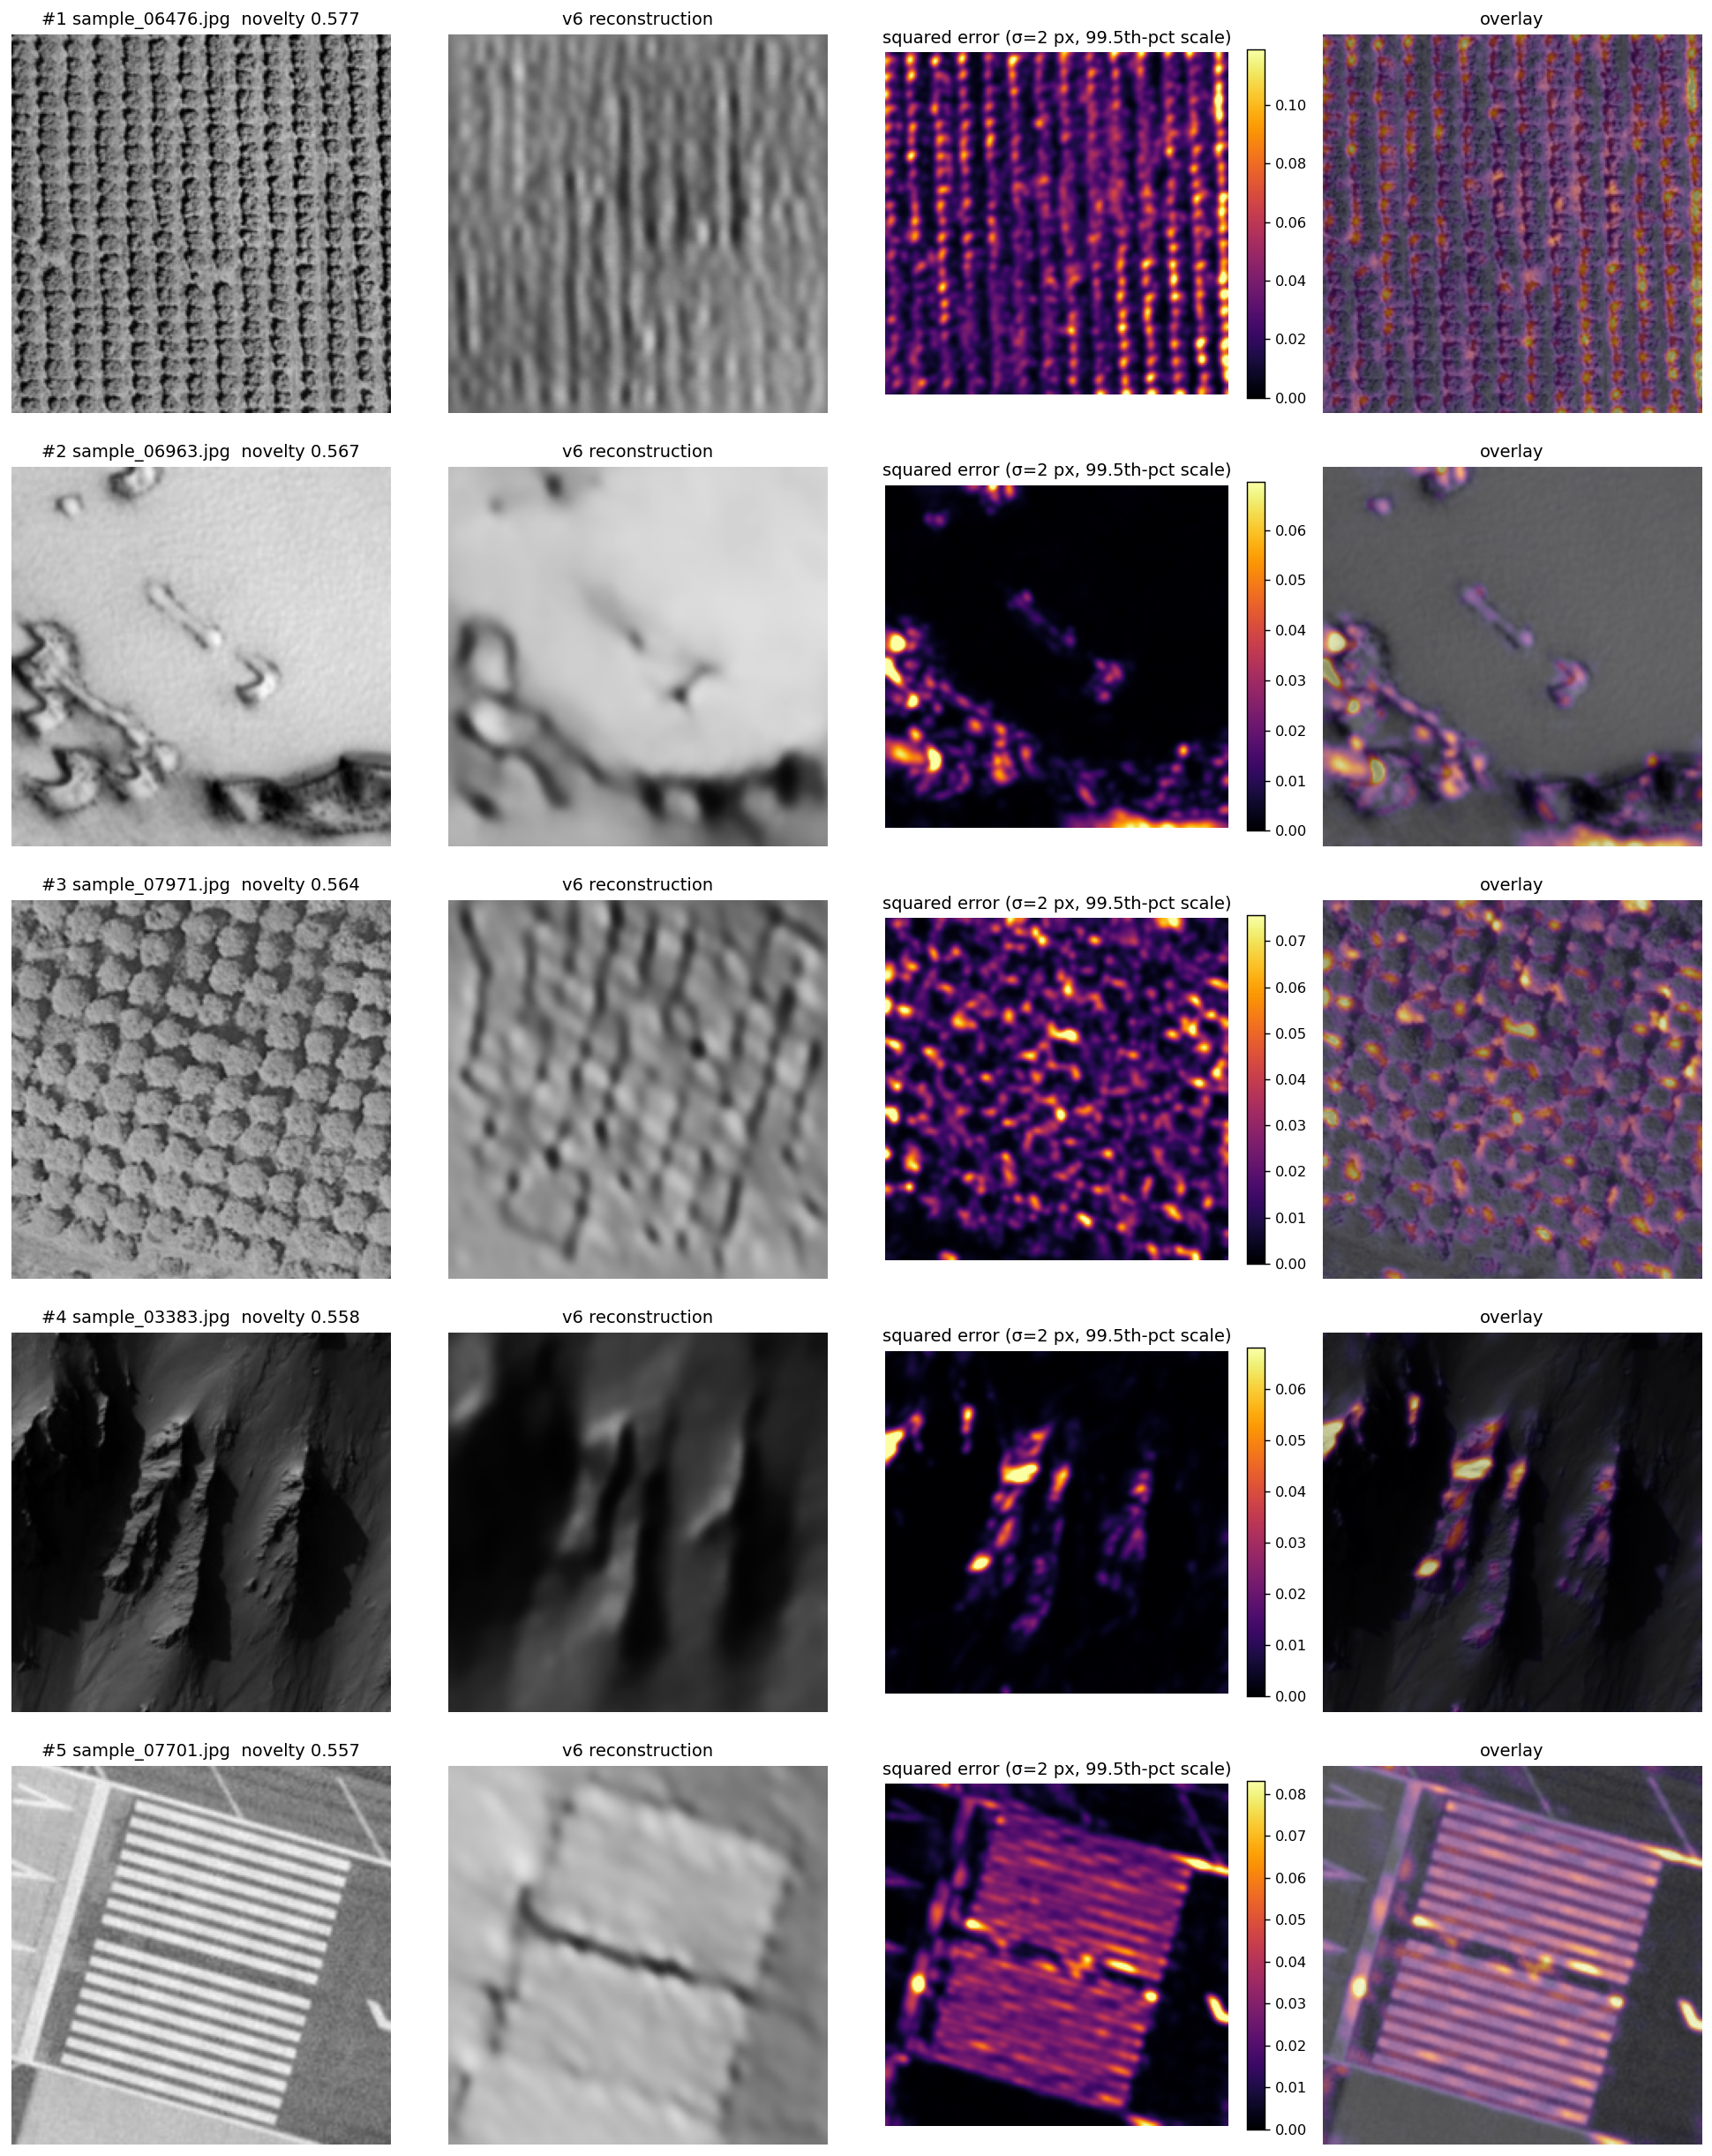
\includegraphics[width=0.74\textwidth]{fig11_heatmaps_top5.png}
\caption{Top-5 thresholded crops: original, stage-1 reconstruction, smoothed squared error (robust colour scale) and overlay.}
\label{fig:hm}
\end{figure*}

\begin{table}[!t]
\centering
\caption{Top-5 crops: Novelty Score, reconstruction MSE and descriptor percentiles vs.\ 500 normal crops}
\label{tab:top5}
\setlength{\tabcolsep}{3pt}
\footnotesize
\begin{tabular}{@{}clccccc@{}}
\toprule
\# & Crop & Source & Nov. & MSE & Conc. & Seam \\
\midrule
1 & 06476 & SRC\_158 & 0.577 & 0.0295 & 2 & 58 \\
2 & 06963 & SRC\_166 & 0.567 & 0.0051 & 88 & 100 \\
3 & 07971 & SRC\_078 & 0.564 & 0.0157 & 5 & 86 \\
4 & 03383 & SRC\_067 & 0.558 & 0.0033 & 96 & 81 \\
5 & 07701 & SRC\_136 & 0.557 & 0.0170 & 3 & 100 \\
\bottomrule
\end{tabular}
\end{table}

\emph{06476 (\#1): orchard-like lattice.} Straight rows of rounded, shadow-casting blobs, a geometry no
Martian process produces at this scale; the error covers every blob (concentration at the 2nd percentile)
and the reconstruction error is at the dataset's 100th percentile: a non-Martian domain shift.
\emph{06963 (\#2): polar knobs.} A bright plain with dark angular knobs in the $90^\circ$N bin; error
concentrated on the dark relief and low overall: rare genuine polar terrain. \emph{07971 (\#3): tree
canopy.} Densely packed rounded crowns; diffuse whole-frame error and high reconstruction error, as for \#1.
\emph{03383 (\#4): low-sun ridges.} A very dark frame whose error sits on the thin sunlit crests: rare but
Martian relief under oblique illumination. \emph{07701 (\#5): stripe markings.} Evenly spaced bright bars
inside rectangles beside straight lines (runway-like painted geometry); error along every bar, high
reconstruction error: foreign content, lifted into the top 5 by the residual code.

Beyond the top five (Fig.~\ref{fig:supp}), the Pentagon photograph ranks 6th with diffuse error,
whereas a black bar and two streaks (ranks 344 and 2,517) still lie in the top 1.5\,\% of
reconstruction error with error along the defect: the synthetic-artefact signature, partly hidden from the latent.
\begin{figure}[!t]
\centering
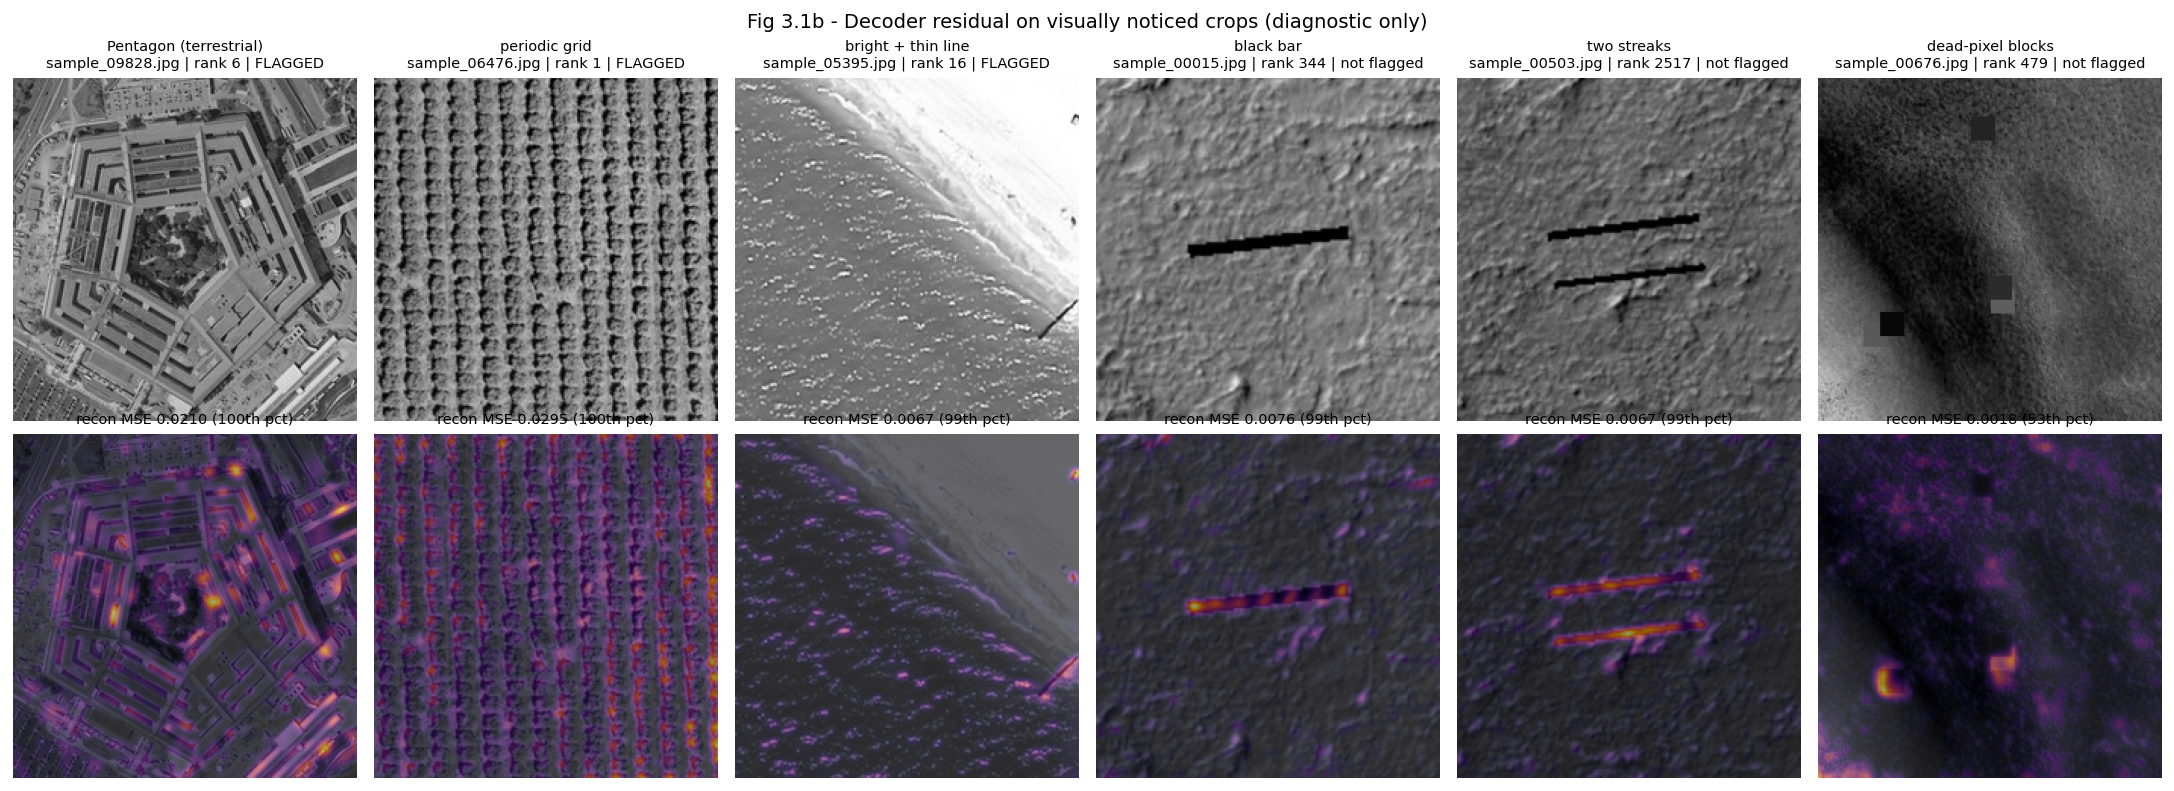
\includegraphics[width=\columnwidth]{fig11b_supplementary_heatmaps.png}
\caption{Decoder residual on visually noticed crops: diffuse error on terrestrial content (left); error along the defect for synthetic glitches (right).}
\label{fig:supp}
\end{figure}

\section{Limitations}
Recall is incomplete: an aerial-buildings image (05508) ranks 156th, and thin streaks and dead-pixel
blocks are missed by latent-space scoring. Rare genuine terrain competes with injected content in the tail.
The no-data mask could hide a genuine defect that touches the crop border (e.g.\ a full-width dark band);
v1/v2 validation metrics include no-data pixels while v3+ use valid pixels only; results are reproducible
up to residual GPU non-determinism; and the planted-fakes benchmark is a proxy.

\section{Conclusion}
A diagnosed data issue (map-projection no-data) and a residual-aware latent mattered more than loss or
bottleneck tweaks. The final two-stage CAE with a latent-space Isolation Forest and a robust, count-free
threshold flags 48 crops; four of its top six are Earth-like images, and heatmap patterns plus metadata
separate injected content from rare Martian geology. Patch-level scoring for small defects is the natural
next step.

\begin{thebibliography}{99}
\bibitem{mcewen2007} A.~S. McEwen \emph{et al.}, ``Mars Reconnaissance Orbiter's High Resolution Imaging Science Experiment (HiRISE),'' \emph{J. Geophys. Res.}, vol.~112, no.~E5, 2007.
\bibitem{doran2020} G.~Doran, E.~Dunkel, S.~Lu, and K.~Wagstaff, ``Mars orbital image (HiRISE) labeled data set version 3.2,'' Zenodo, 2020.
\bibitem{hinton2006} G.~E. Hinton and R.~R. Salakhutdinov, ``Reducing the dimensionality of data with neural networks,'' \emph{Science}, vol.~313, no.~5786, pp.~504--507, 2006.
\bibitem{loshchilov2019} I.~Loshchilov and F.~Hutter, ``Decoupled weight decay regularization,'' in \emph{Proc. ICLR}, 2019.
\bibitem{wang2004} Z.~Wang, A.~C. Bovik, H.~R. Sheikh, and E.~P. Simoncelli, ``Image quality assessment: From error visibility to structural similarity,'' \emph{IEEE Trans. Image Process.}, vol.~13, no.~4, pp.~600--612, 2004.
\bibitem{zhao2017} H.~Zhao, O.~Gallo, I.~Frosio, and J.~Kautz, ``Loss functions for image restoration with neural networks,'' \emph{IEEE Trans. Comput. Imag.}, vol.~3, no.~1, pp.~47--57, 2017.
\bibitem{liu2008} F.~T. Liu, K.~M. Ting, and Z.-H. Zhou, ``Isolation forest,'' in \emph{Proc. IEEE ICDM}, 2008, pp.~413--422.
\bibitem{iglewicz1993} B.~Iglewicz and D.~C. Hoaglin, \emph{How to Detect and Handle Outliers}. Milwaukee, WI, USA: ASQC Quality Press, 1993.
\bibitem{dagostino1971} R.~B. D'Agostino, ``An omnibus test of normality for moderate and large size samples,'' \emph{Biometrika}, vol.~58, no.~2, pp.~341--348, 1971.
\bibitem{satopaa2011} V.~Satop\"a\"a, J.~Albrecht, D.~Irwin, and B.~Raghavan, ``Finding a `kneedle' in a haystack: Detecting knee points in system behavior,'' in \emph{Proc. ICDCS Workshops}, 2011, pp.~166--171.
\bibitem{vandermaaten2008} L.~van der Maaten and G.~Hinton, ``Visualizing data using t-SNE,'' \emph{J. Mach. Learn. Res.}, vol.~9, pp.~2579--2605, 2008.
\end{thebibliography}

\end{document}
